\documentclass[11pt]{article}

\usepackage[a4paper,margin=3cm]{geometry} % For page dimensions
\usepackage{fontspec} % For font selection
\usepackage{unicode-math} % For mathematical fonts
\usepackage{polyglossia} % For language selection
\usepackage{graphicx} % For images
\usepackage[colorlinks=true, linkcolor=black, urlcolor=blue, citecolor=green]{hyperref} % For hyperlinks
\usepackage{xcolor} % Colors for code highlighting
\usepackage{fancyhdr} % For headers and footers
\usepackage{bookmark}
\usepackage{nameref} % For referencing sections
\usepackage{draftwatermark} % For watermarks
\usepackage{amsmath} % For mathematical equations
\usepackage{listings} % For code formattings
\usepackage{tikz} % For diagrams

\graphicspath{ {images} }

% Set fonts
% \setmainfont{Noto Serif}
\setromanfont{Noto Serif}
\setsansfont{Noto Sans}
\setmonofont{Noto Sans Mono}

% Set languages
\setmainlanguage{greek}
\setotherlanguages{english}

% Header and footer settings
\pagestyle{fancy}
\setlength{\headheight}{14pt}
\fancyhf{}
\fancyfoot[C]{\thepage}

% Custom Commands
\newcommand{\email}[1]{\href{mailto://#1}{\texttt{#1}}} % Email formatting
\newcommand{\developer}[2]{#1 (#2) \\ \email{up#2@ac.upatras.gr} \\[2ex]}
\newcommand{\appname}{Loop}

\author{
    \developer{Γιάννης Ραβασόπουλος}{1100696}
    \developer{Κώστας Λουκανάρης}{1100610}
    \developer{Χρήστος Μάριος Νικολόπουλος}{1100644}
    \developer{Άγγελος Αβεντισιάν}{1100491}
    \developer{Βασίλης Μυλωνάς}{1100643}
}

\date{
    \today \\[1ex]
    Έκδοση 0.1 \\
}


\fancyhead[L]{Περιγραφή Έργου}
\fancyhead[R]{\leftmark}

\title{
    Περιγραφή Έργου - \appname\\[1ex]
    \large Τεχνολογία Λογισμικού - ΤΜΗΥΠ, Πανεπιστήμιο Πατρών \\[2ex]
}

\begin{document}

\maketitle
\thispagestyle{empty}
\newpage

\tableofcontents
\newpage

\begin{abstract}
    Περιγραφή ανάπτυξης συστήματος και συνοδεύουσας εφαρμογής για την διευκόλυνση
    συνεπιβίβασης σε κοινές διαδρομές (carpooling). Η εφαρμογή εγκαθισταται σε
    κινητές συσκευές και παρέχει ζωντανή πληροφόρηση
    αντλώντας πληροφορίες από τους χρήστες. H εφαρμογή απευθύνεται αμφότερα σε
    οδηγούς αυτοκινήτων αλλά και σε πεζούς. Στόχος είναι η καλύτερη αξιοποίηση
    του οδικού δικτύου και η μείωση της κυκλοφοριακής συμφόρησης σε αστικές
    περιοχές.
\end{abstract}

\newpage

\section{Περιγραφή}

\subsection{Περιγραφή του Προβλήματος}

Είναι γνωστό ότι το μεγαλύτερο μέρος του αστικού πληθυσμού είναι άτομα τα
οποία έχουν καθημερινές υποχρεώσεις και πρέπει να βρίσκονται
σε συγκεκριμένα μέρη σε συγκεκριμένες ώρες. Χαρακτηριστικό παράδειγμα είναι οι
φοιτητές και οι εργαζόμενοι οι οποίοι έχουν συνήθως προκαθορισμένο ωράριο και
πρόγραμμα.

Πολλοί από αυτούς επιλέγουν την αυτοκίνηση λόγω της κακής κατάστασης των μέσων
μαζικής μεταφοράς. Ενδεικτικά είναι τα λεωφορεία με δρομολόγια
προς το πανεπιστήμιο τα οποία είναι γεμάτα τις πρωινές ώρες. Η αύξηση όμως της
χρήσης των αυτοκινήτων οδηγεί σε αύξηση της κυκλοφοριακής συμφόρησης και
της ατμοσφαιρικής ρύπανσης.

\subsection{Προτεινόμενη Λύση}

Η προτεινόμενη λύση είναι η ανάπτυξη μίας εφαρμογής για κινητές συσκευές
η οποία θα διευκολύνει τους χρήστες να μοιράζονται οχήματα (carpooling) στις
διαδρομές τους. Μοιράζοντας οχήματα σε κοινές διαδρομές η χρήστες μειώνουν
την κυκλοφοριακή συμφόρηση και ταυτόχρονα το κόστος μεταφοράς τους.

Σαν επιπλέον όφελος προτείνεται η υλοποίηση ενός συστήματος πόντων και ανταμοιβών
υπό την μορφή κουπονιών το οποίο θα ενθαρρύνει τους χρήστες να συμμετάσχουν
στην εφαρμογή.

\newpage

\section{Σύσταση Ομάδας}
Η ομάδα αποτελείται από 5 μέλη, με ρόλους που καθορίστηκαν βάσει της εμπειρίας και των ενδιαφερόντων:
\begin{itemize}
    \item Βασίλης Μυλωνάς (Επικεφαλής Έργου / Project Manager)
    \item Άγγελος Αβεντισιάν (Υπεύθυνος Ποιότητας / QA Manager)
    \item Γιάννης Ραβασόπουλος
    \item Κώστας Λουκανάρης
    \item Χρήστος Μάριος Νικολόπουλος
\end{itemize}

\newpage

\section{Απαιτήσεις}

\subsection{Λειτουργικές Απαιτήσεις}

\begin{enumerate}
    \item Ο χρήστης πρέπει να μπορεί να εγγραφεί και να συνδεθεί μέσω πολλαπλών μεθόδων (email, Google, Facebook).
    \item Ο χρήστης πρέπει να μπορεί να δηλώνει δραστηριότητες, παρέχοντας πληροφορίες όπως τοποθεσία και ώρες.
    \item Να υπάρχει η δυνατότητα αναζήτησης άλλων χρηστών με όμοιες διαδρομές.
    \item Να δίνεται η δυνατότητα επικοινωνίας μεταξύ των χρηστών για τον καθορισμό σημείου συνάντησης.
    \item Να εφαρμόζεται σύστημα βαθμολόγησης και σχολιασμού, τόσο για οδηγούς όσο και για επιβάτες.
    \item Η εφαρμογή θα πρέπει να παρέχει ανταμοιβές υπό τη μορφή κουπονιών ως κίνητρο χρήσης.
\end{enumerate}

\subsection{Μη Λειτουργικές Απαιτήσεις}

\begin{enumerate}
    \item Η αναζήτηση και οι ενημερώσεις δεδομένων θα πρέπει να γίνονται σε πραγματικό χρόνο.
    \item Πρέπει να διασφαλίζεται η ασφάλεια των επιβατών και των οδηγών μέσω ελέγχου ταυτότητας
          και επαλήθευσης χρηστών.
    \item Το σύστημα πρέπει να υποστηρίζει μελλοντικές επεκτάσεις με πρόσθεση νέων λειτουργιών.
    \item Η διεπαφή θα πρέπει να είναι φιλική και εύχρηστη για όλους τους χρήστες.
\end{enumerate}

\newpage

\section{Ενδεικτικές Οθόνες}

\subsection{Κεντρική Οθόνη}

\begin{figure}[H]
    \centering
    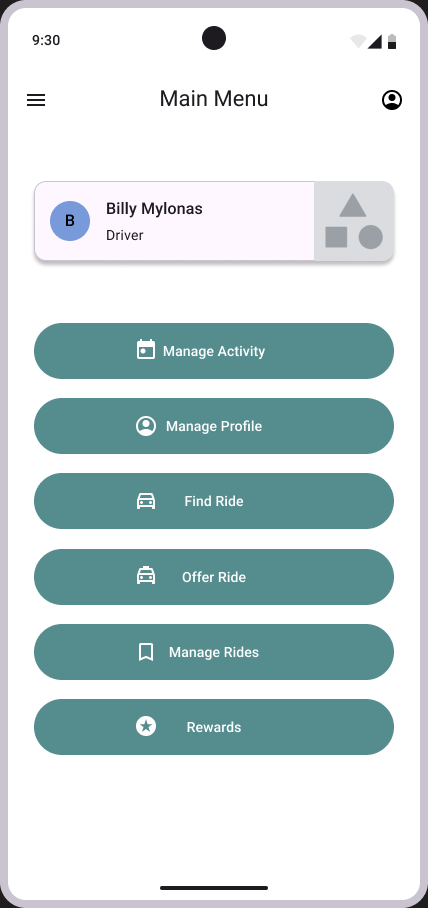
\includegraphics[width=0.9\textwidth]{mockups/main-menu}
    \caption{Κεντρική Οθόνη}
\end{figure}

\subsection{Εύρεση Διαδρομής (Find Ride)}

\begin{figure}[H]
    \centering
    \begin{subfigure}[b]{0.28\textwidth}
        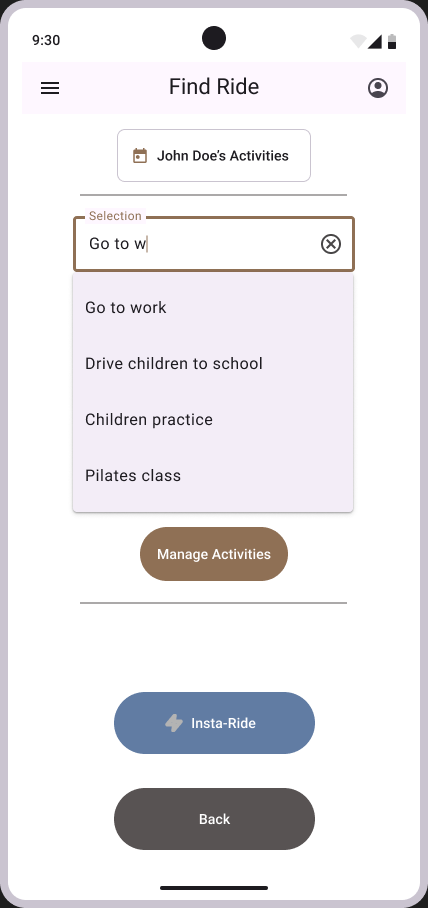
\includegraphics[width=\textwidth]{mockups/find-ride-1}
        \caption{Επιλογή διαδρομής μέσω Activity}
    \end{subfigure}
    \hfill
    \begin{subfigure}[b]{0.28\textwidth}
        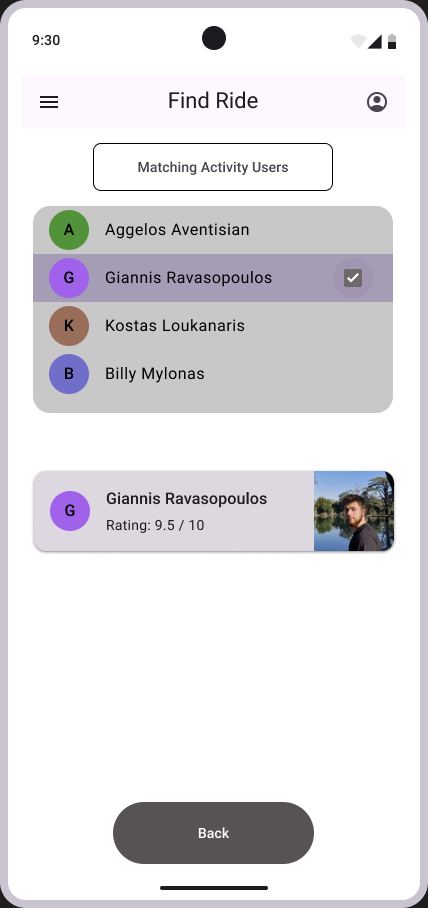
\includegraphics[width=\textwidth]{mockups/find-ride-2}
        \caption{Επιλογή συνεπιβατών}
    \end{subfigure}
    \hfill
    \begin{subfigure}[b]{0.28\textwidth}
        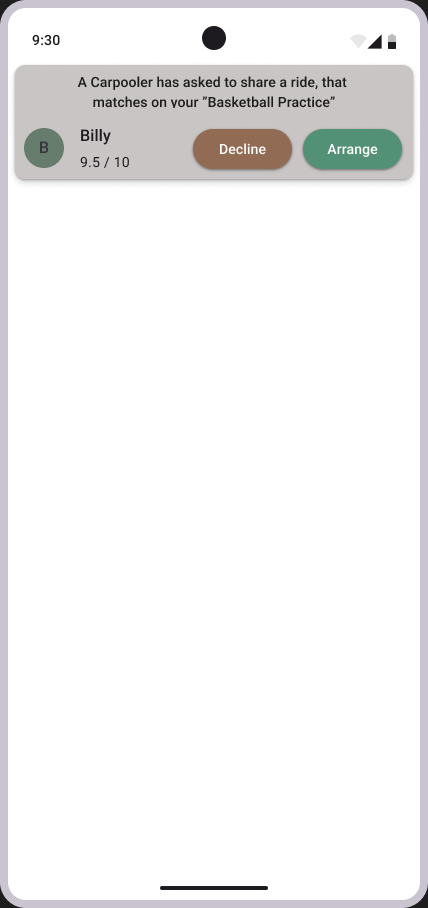
\includegraphics[width=\textwidth]{mockups/find-ride-3}
        \caption{Ειδοποίηση οδηγού}
    \end{subfigure}
    \caption{Διαδικασία εύρεσης διαδρομής}
\end{figure}

\begin{figure}[H]
    \centering
    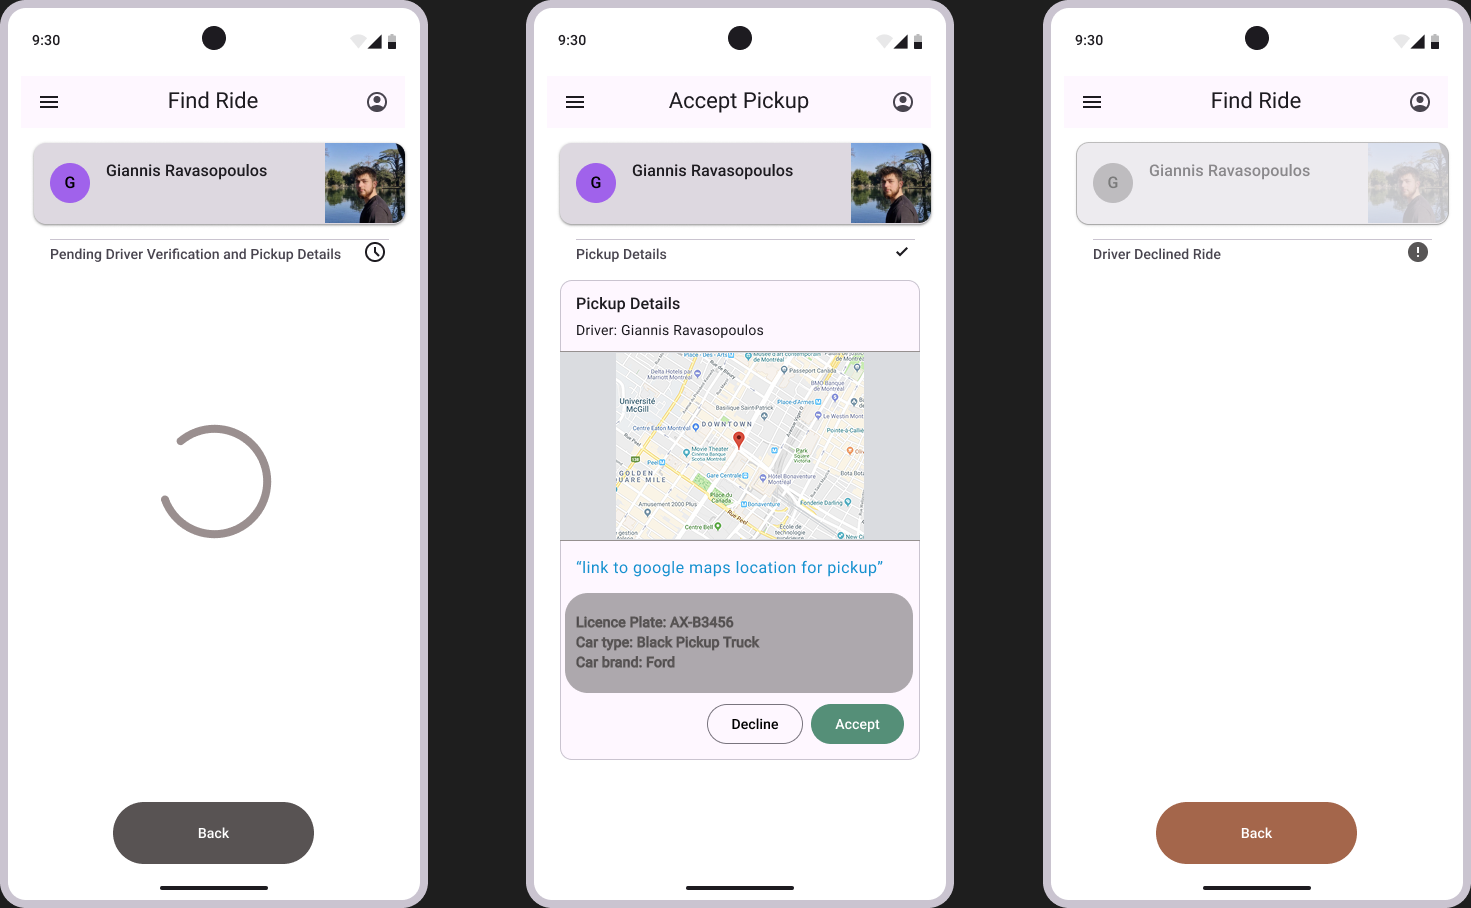
\includegraphics[width=0.9\textwidth]{mockups/find-ride-4}
    \caption{Επιβεβαίωση σημείου παραλαβής (2: σενάριο αποδοχής από τον οδηγό, 3: σενάριο απόρριψης από τον οδηγό)}
\end{figure}

\newpage

\begin{figure}[H]
    \centering
    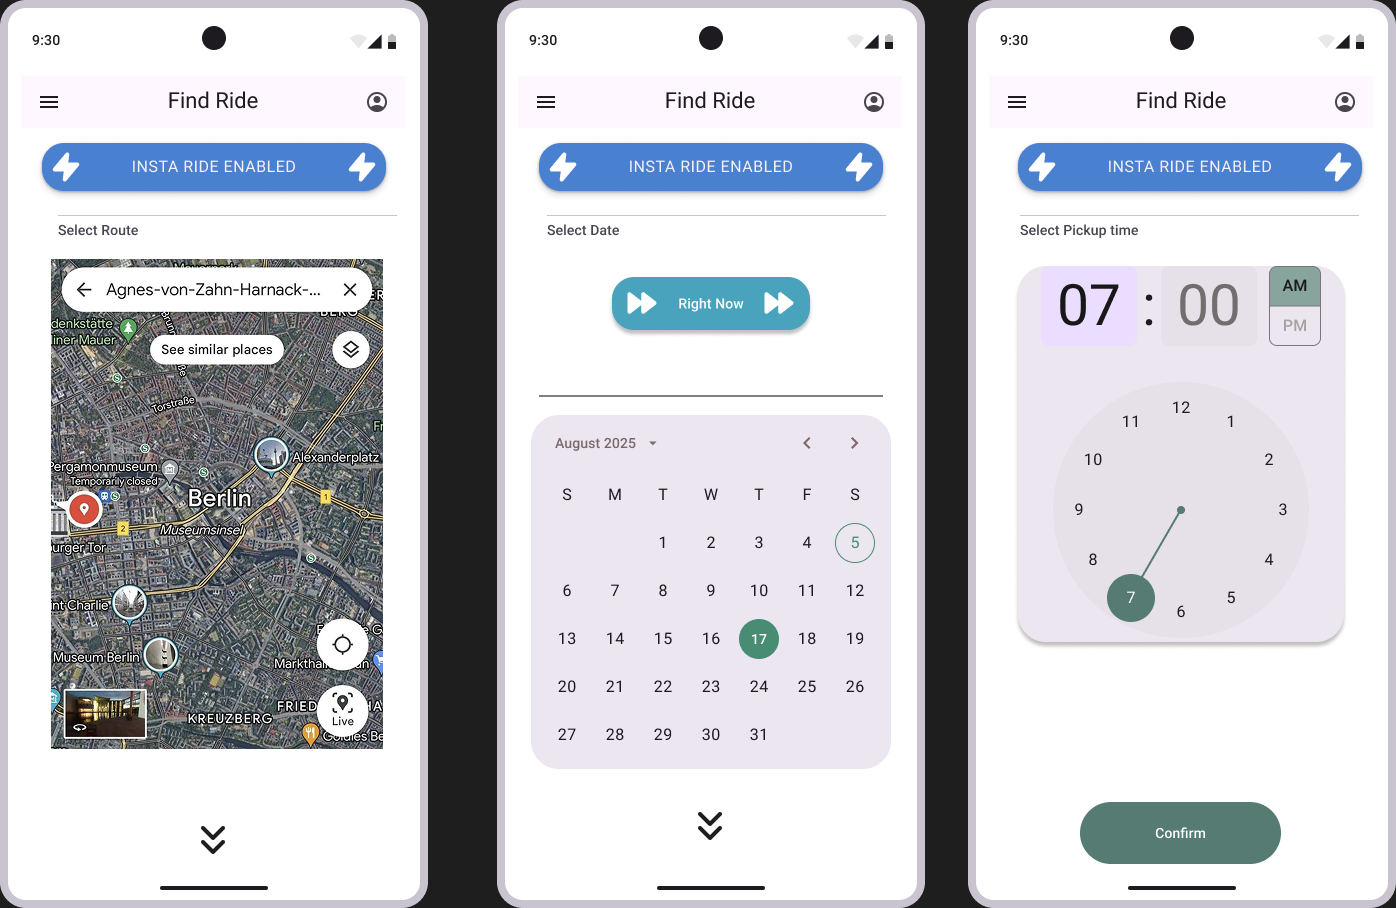
\includegraphics[width=\textwidth]{mockups/find-ride-1b}
    \caption{Επιλογή διαδρομής μέσω Insta-Ride}
\end{figure}

\newpage

\subsection{Προσφορά Διαδρομής (Offer Ride)}

\begin{figure}[H]
    \centering
    \begin{subfigure}[b]{0.3\textwidth}
        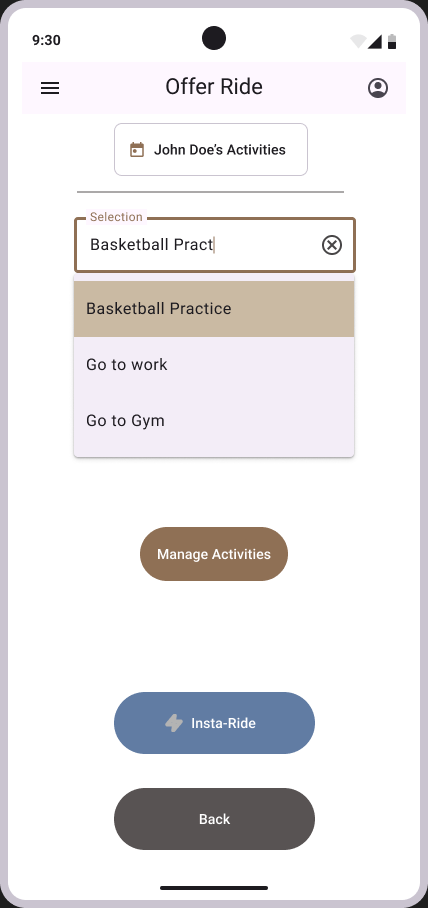
\includegraphics[width=\textwidth]{mockups/offer-ride-1}
        \caption{Επιλογή διαδρομής μέσω Activity}
    \end{subfigure}
    \hfill
    \begin{subfigure}[b]{0.3\textwidth}
        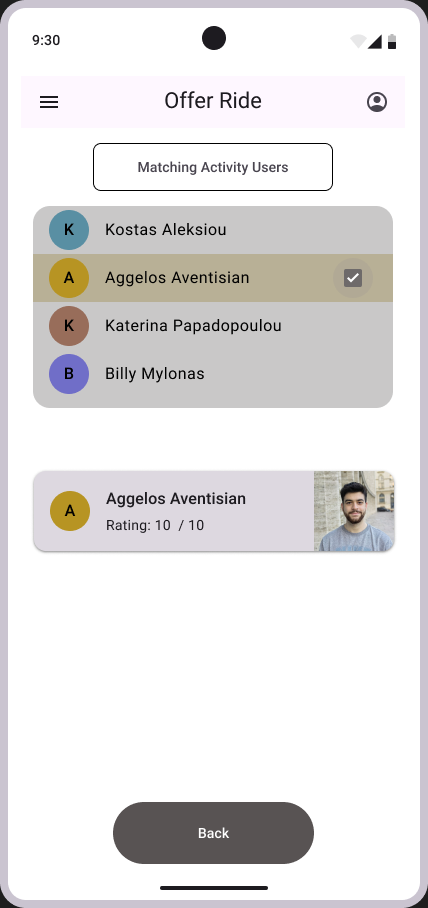
\includegraphics[width=\textwidth]{mockups/offer-ride-2}
        \caption{Επιλογή οδηγού}
    \end{subfigure}
\end{figure}

\begin{figure}[H]
    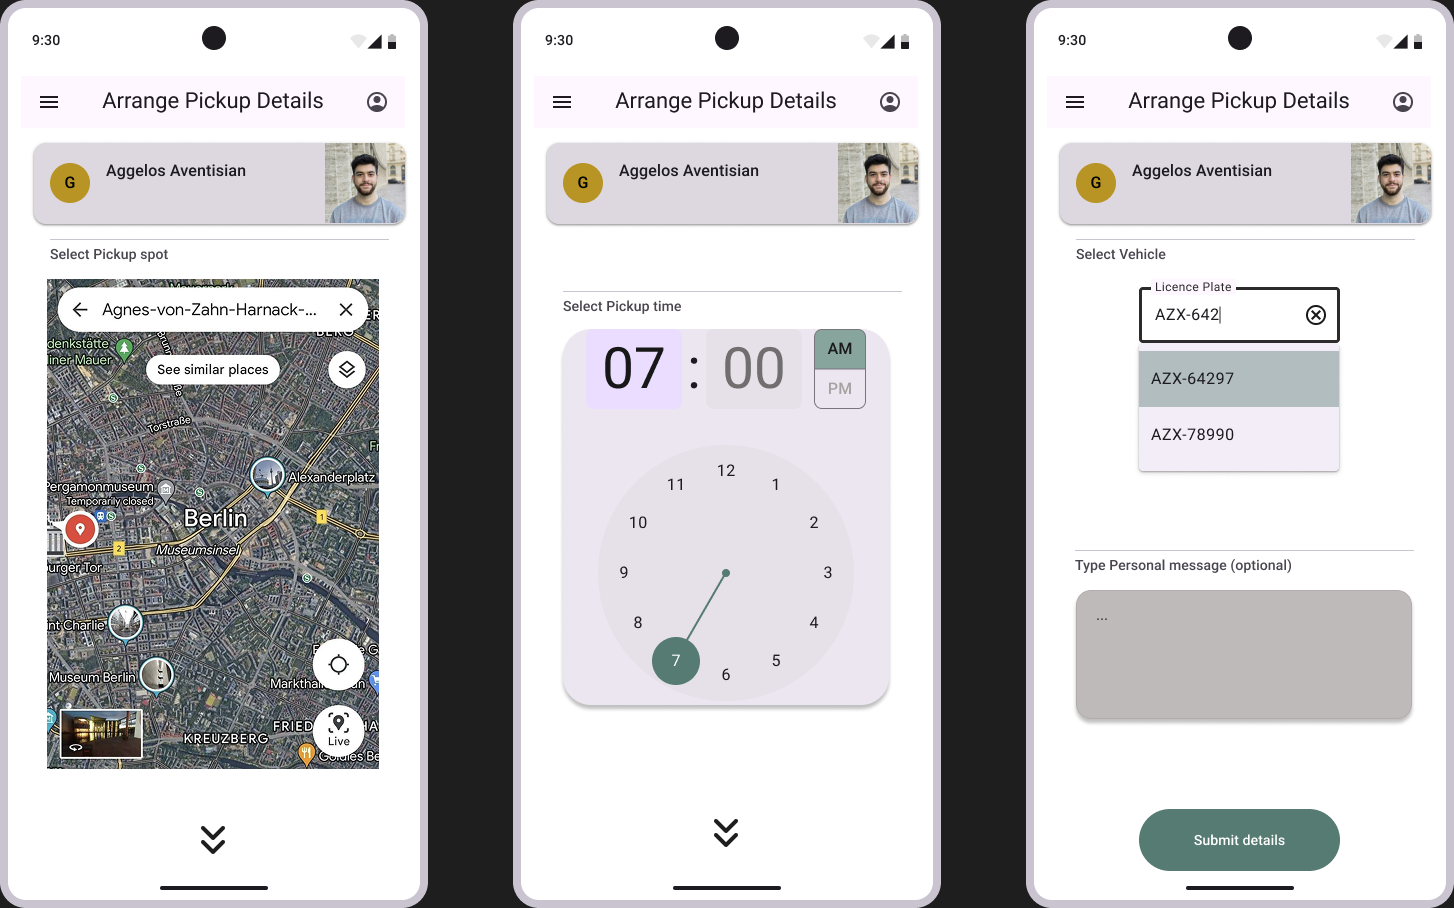
\includegraphics[width=0.9\textwidth]{mockups/offer-ride-3a}
    \caption{Επιλογή σημείου και ώρας παραλαβής}
\end{figure}

\newpage

\begin{figure}[h!]
    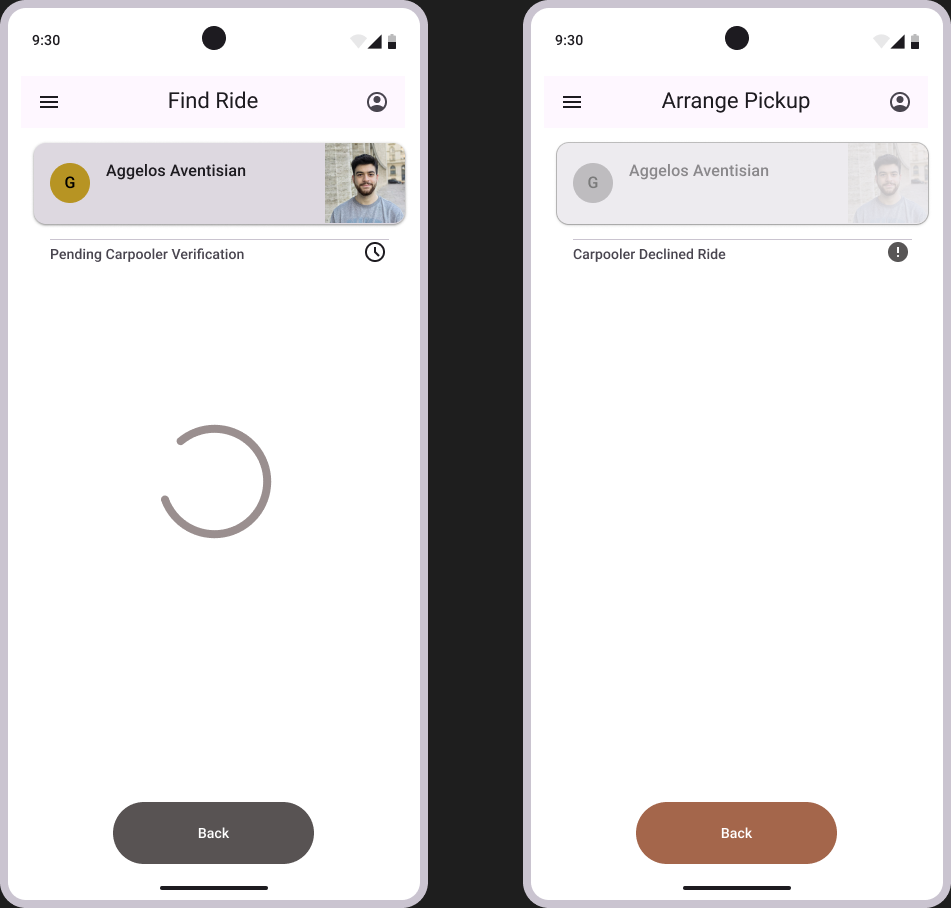
\includegraphics[width=\textwidth]{mockups/offer-ride-3b}
    \caption{Απόρριψη από τον Carpooler}
\end{figure}

\newpage

\subsection{Manage Ride}

\begin{figure}[H]
    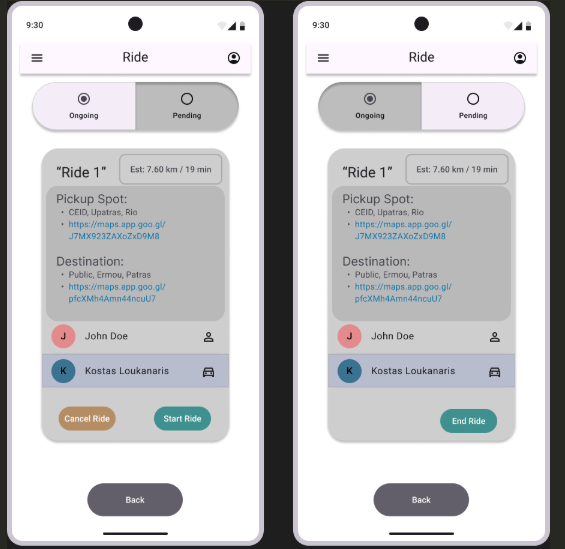
\includegraphics[width=\textwidth]{mockups/image}
    \caption{Έναρξη διαδρομής (Start Ride)}
\end{figure}

\newpage

\subsection{Εξαργύρωση ανταμοιβής (Redeem Reward)}

\begin{figure}[H]
    \centering
    \begin{subfigure}[b]{0.3\textwidth}
        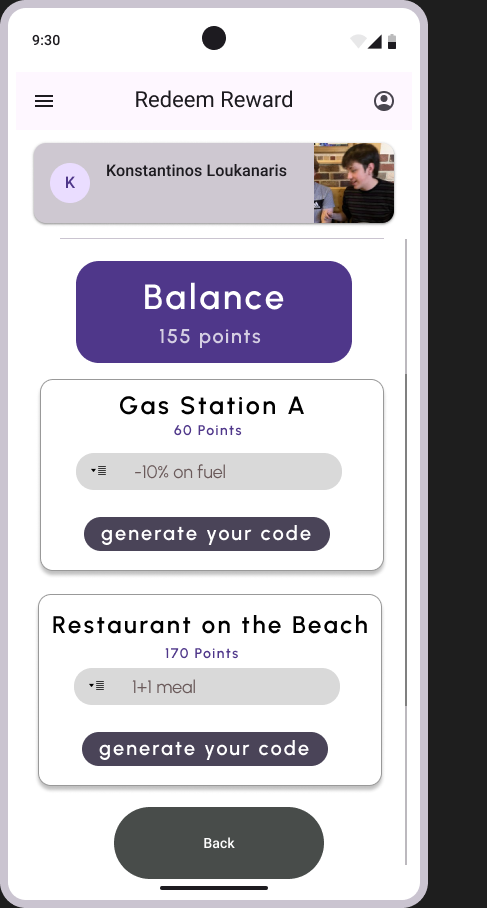
\includegraphics[width=\textwidth]{mockups/redeem-reward-3}
        \caption{Εμφάνιση Κουπονιών και πόντων}
    \end{subfigure}
    \hfill
    \begin{subfigure}[b]{0.3\textwidth}
        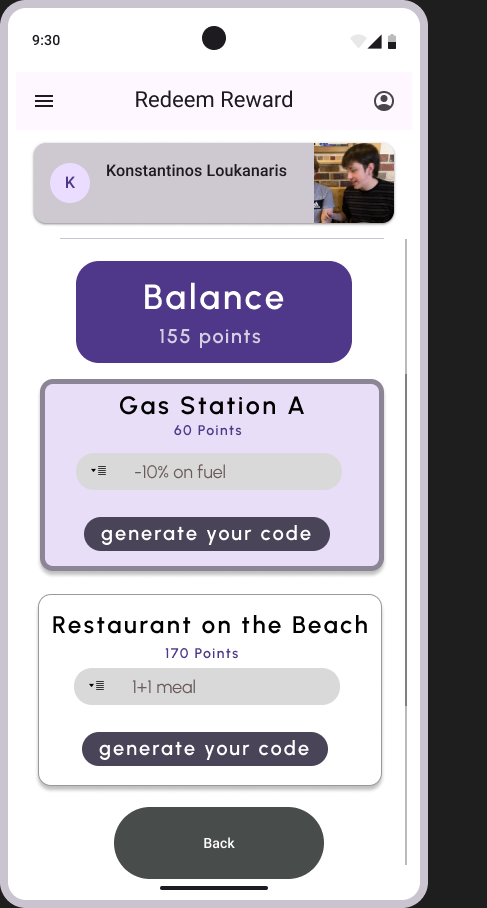
\includegraphics[width=\textwidth]{mockups/redeem-reward-4}
        \caption{Επιλογή κουπονιού}
    \end{subfigure}
    \hfill
    \begin{subfigure}[b]{0.3\textwidth}
        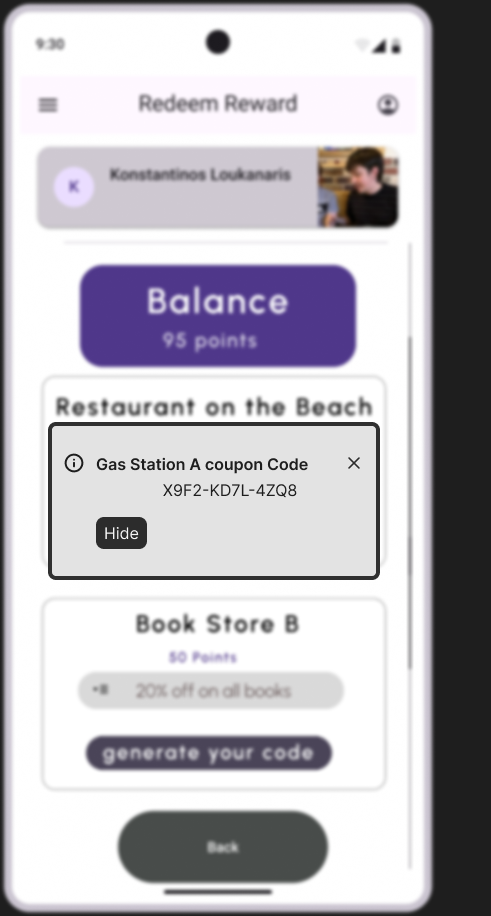
\includegraphics[width=0.9\textwidth]{mockups/redeem-reward-5}
        \caption{Επιβεβαίωση εξαργύρωσης και εμφάνιση κωδικού κουπονιού}
    \end{subfigure}
\end{figure}

\newpage

\subsection{Λοιπές Οθόνες}

\begin{figure}[H]
    \centering
    \begin{subfigure}[b]{0.3\textwidth}
        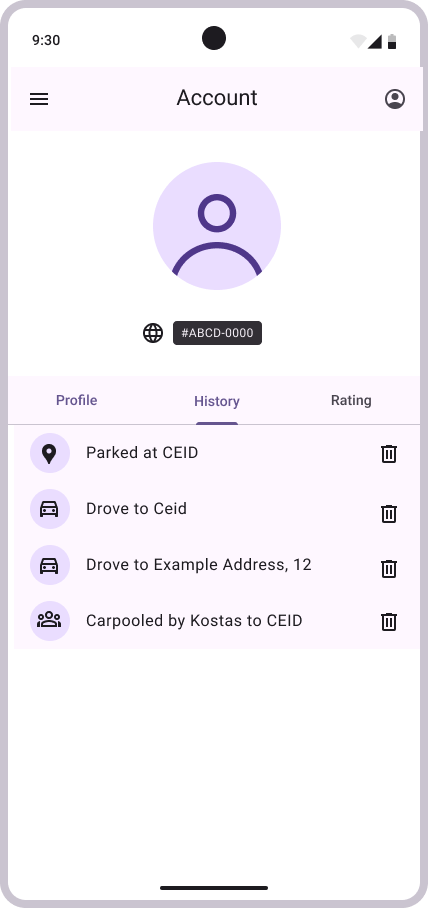
\includegraphics[width=\textwidth]{mockups/history}
        \caption{Προβολή Ιστορικού}
    \end{subfigure}
    \hfill
    \begin{subfigure}[b]{0.3\textwidth}
        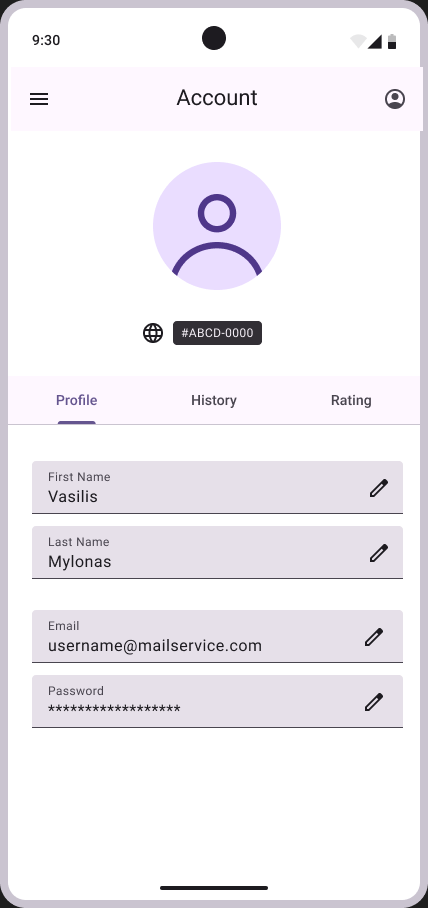
\includegraphics[width=\textwidth]{mockups/profile}
        \caption{Προβολή Προφίλ}
    \end{subfigure}
    \hfill
    \begin{subfigure}[b]{0.3\textwidth}
        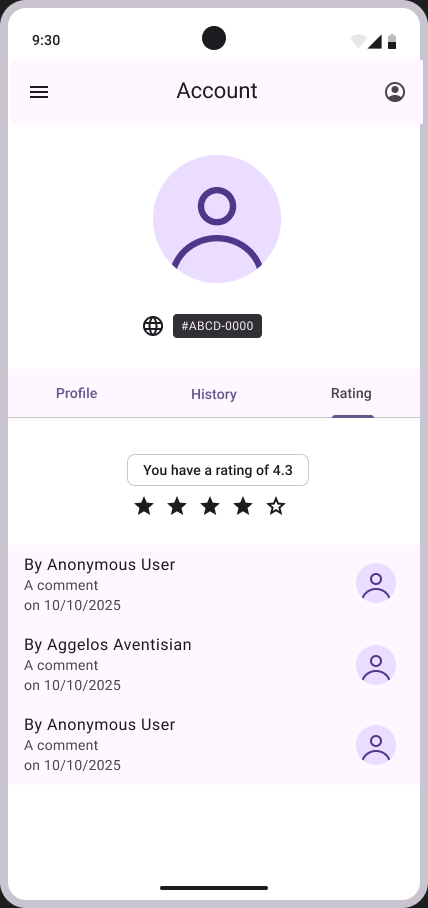
\includegraphics[width=\textwidth]{mockups/rating}
        \caption{Προβολή Βαθμολογίας}
    \end{subfigure}
    \caption{}
\end{figure}

\end{document}
